\lecture{9}{13 Nov. 14:20}{}

\section{All-Pairs Shortest Path Problem}

\begin{problem}[All-Pairs Distance Problem]
    Given
    \begin{itemize}
        \item Input: an edge-weighted directed graph $G$ with $V(G) = \{1, 2, \cdots, n\}$ edge weights $w: E(G) \to \mathbb{R}^+$, without negative cycles.
        \item Output: $d_G(i,j)$ for all $i,j \in V(G)$.
    \end{itemize}
\end{problem}

\begin{figure}[H]
    \centering
    
    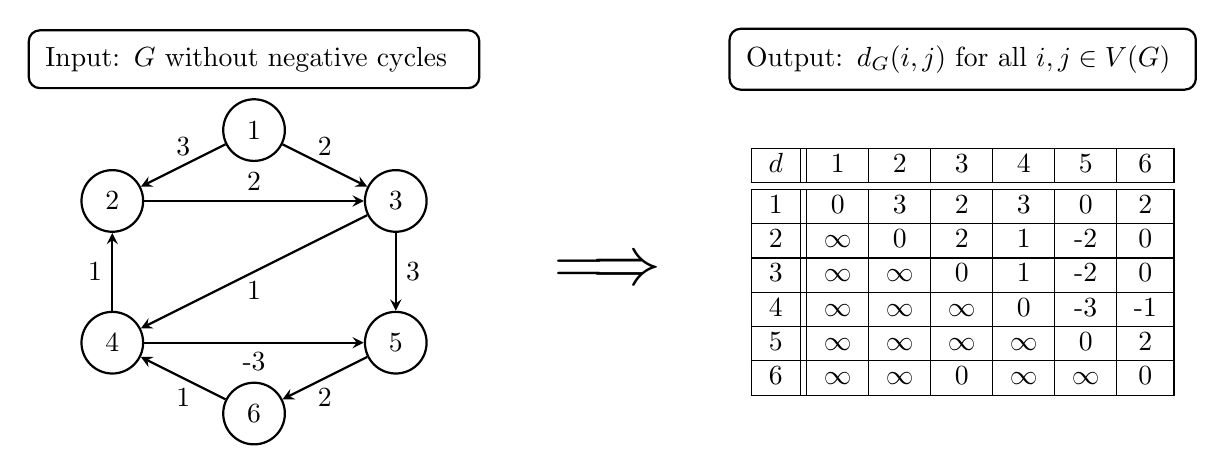
\begin{tikzpicture}[>=stealth,thick,scale=0.9]
    
    % ============================
    % Left Side: Graph
    % ============================
    
    \tikzstyle{vtx}=[circle,draw=black,fill=white,inner sep=5pt]
    
    \node[rectangle,rounded corners,draw=black,fill=white,
            inner sep=6pt,text width=5.3cm] 
            at (0,3)
            {Input: $G$ without negative cycles};
    
    \node[vtx] (1) at (0,2) {1};
    \node[vtx] (2) at (-2,1) {2};
    \node[vtx] (3) at (2,1) {3};
    \node[vtx] (4) at (-2,-1) {4};
    \node[vtx] (5) at (2,-1) {5};
    \node[vtx] (6) at (0,-2) {6};
    
    % Black edges
    \draw[->] (1) -- node[midway,above]{3} (2);
    \draw[->] (2) -- node[midway,above]{2} (3);
    \draw[->] (3) -- node[midway,right]{3} (5);
    \draw[->] (5) -- node[midway,below]{2} (6);
    \draw[->] (6) -- node[midway,below]{1} (4);
    \draw[->] (4) -- node[midway,left]{1} (2);
    
    % Former yellow edges → black
    \draw[->] (1) -- node[midway,above]{2} (3);
    \draw[->] (3) -- node[midway,below]{1} (4);
    \draw[->] (4) -- node[midway,below]{-3} (5);
    
    \node at (5,0) {\Huge $\Longrightarrow$};
    
    % ============================
    % Right Side: Table
    % ============================
    
    \node[rectangle,rounded corners,draw=black,fill=white,
            inner sep=6pt,text width=5.5cm] 
            at (10,3)
            {Output: $d_G(i,j)$ for all $i,j \in V(G)$};
    
    \node at (10,0) {%
    \begin{tabular}{|c||c|c|c|c|c|c|}
    \hline
    $d$ & 1 & 2 & 3 & 4 & 5 & 6 \\ \hline
    \hline
    1 & 0 & 3 & 2 & 3 & 0 & 2 \\ \hline
    2 & $\infty$ & 0 & 2 & 1 & -2 & 0 \\ \hline
    3 & $\infty$ & $\infty$ & 0 & 1 & -2 & 0 \\ \hline
    4 & $\infty$ & $\infty$ & $\infty$ & 0 & -3 & -1 \\ \hline
    5 & $\infty$ & $\infty$ & $\infty$ & $\infty$ & 0 & 2 \\ \hline
    6 & $\infty$ & $\infty$ & 0 & $\infty$ & $\infty$ & 0 \\ \hline
    \end{tabular}
    };
    \end{tikzpicture}
    \caption{All-Pairs Distance Problem Example}
\end{figure}

\newpage

\begin{idea}[Naive Solution]
    Sloving the single-source shortest path problem for each vertex using Dijkstra, Lawler, or  Bellman-Ford algorithm.
\end{idea}

\subsection{A Naive DP Solution}

\begin{definition}
    Let $w_k(i, j)$ be the length of the shortest $ij$-path in $G$ having at most $k$ edges. It will be $\infty$ if no such path exists.
    \[
        \begin{cases}
            w_1(i, j) &= w(ij) \\
            w_{n-1}(i, j) &= d_G(i, j)
        \end{cases}
    \]
\end{definition}

\begin{idea}
    Use the recurrence relation for $w_k(i, j)$ is
    \[
        \begin{cases}
            w_1(i, j) &= w(ij) \\
            w_{2k}(i, j) &= \displaystyle \min_{1 \leq t \leq n} (w_{k}(i, t) + w_k(t, j))
        \end{cases}
    \]
    \begin{itemize}
        \item For each $(i, j, k)$, take $O(n)$ time to compute $w_{2k}(i, j)$ from $w_k(i, j)$.
        \item For each $k$, there are $n^2$ pairs of $(i, j)$, using $O(n^3)$ time to compute all $w_{2k}$ from all $w_k$.
        \item It take $O(\log n)$ iterations to compute $d_G = w_{n-1}$ from $w_1$.
    \end{itemize}
    \begin{note}
        The running time is $O(n^3 \log n)$.
    \end{note}
\end{idea}

\subsection{Floyd and Warshall's DP algorithm}

\begin{definition}
    Let $d_k(i, j)$ be the length of the shortest $ij$-path in $G$ whose intermediate vertices are at most $k$. It will be $\infty$ if no such path exists.
    \[
        \begin{cases}
            d_0(i, j) &= w(ij) \\
            d_{n}(i, j) &= d_G(i, j)
        \end{cases}
    \]
\end{definition}

\[
\begin{tikzpicture}[>=stealth, node distance=1.8cm]
\tikzstyle{node}=[circle, draw=black, fill=white,
                  minimum size=16pt, inner sep=0pt]

\node[node] (i) {$i$};
\node[node] (a) [right of=i] {};
\node[node] (b) [right of=a] {};
\node[node] (c) [right of=b] {$k$};
\node[node] (d) [right of=c] {};
\node[node] (e) [right of=d] {};
\node[node] (j) [right of=e] {$j$};

\draw[->] (i) -- (a);
\draw[->] (a) -- (b);
\draw[->] (b) -- (c);
\draw[->] (c) -- (d);
\draw[->] (d) -- (e);
\draw[->] (e) -- (j);

% 下方兩個 underbrace
\node at ($(c) - (3.5,0.8)$)
    {$\underbrace{\hspace{3.7cm}}_{\text{indices at most } k-1}$};

\node at ($(d)!0.5!(j) - (0,0.8)$)
    {$\underbrace{\hspace{3.1cm}}_{\text{indices at most } k-1}$};

\end{tikzpicture}
\]

\begin{idea}[Floyd and Warshall's DP Algorithm]
    Using the recurrence relation for $d_k(i, j)$ is
    \[
        \begin{cases}
            d_0(i, j) &= w(ij) \\
            d_{k}(i, j) &= \min\{d_{k-1}(i, j),\ d_{k-1}(i, k) + d_{k-1}(k, j)\}
        \end{cases}
    \]
    \begin{itemize}
        \item For each $(i, j, k)$, take $O(1)$ time to compute $d_k(i, j)$ from $d_{k-1}(i, j)$.
        \item For each $k$, there are $n^2$ pairs of $(i, j)$, using $O(n^2)$ time to compute all $d_k$ from all $d_{k-1}$.
        \item It take $n$ iterations to compute $d_G = d_n$ from $d_0$.
    \end{itemize}
    \begin{note}
        The running time is $O(n^3)$.
    \end{note}
\end{idea}

\subsection{Johnson's Reweighting Technique}

\begin{idea}[Naive Solution with Dijkstra]
    如果我們可以拿到一個 nonnegative edge-weight 的 graph,我們就可以簡單地用 Dijkstra's algorithm 來解 All-Pairs Shortest Path Problem
    \begin{itemize}
        \item For each vertex $i$ of $G$, run Dijkstra's algorithm + Quake heap in $O(m + n\log n)$ time to compute $d_G(i, j)$ for all $j \in V(G)$.
    \end{itemize}
    \begin{note}
        The running time is $O(nm + n^2\log n)$.
    \end{note}
\end{idea}

\vspace{1em}

所以我們需要一個方法把有負邊權的 graph 轉換成 nonnegative edge-weight 的 graph,Reweighting $w$ into $\hat{w}$ such that
\begin{itemize}
    \item $\hat{w}$ is nonnegative
    \item If $\hat{w}$ is the reweighted shortest $ij$-path, then the original shortest $ij$-path is $w$.
\end{itemize}

\begin{idea}[Johnson's Reweighting Technique]
    Following these steps:
    \begin{itemize}
        \item Assign a weight $h(i)$ to each vertex $i$ of $G$.
        \item Let \[
            \hat{w}(ij) = w(ij) + h(i) - h(j)
        \]
        \item Then for any $ij$-path $P$, we have \[
            \hat{w}(P) = w(P) + h(i) - h(j)
        \]
    \end{itemize}
    \begin{remark}
        $P$ is a shortest $ij$-path in $G$ with respect to $\hat{w}$ if and only if it is a shortest $ij$-path in $G$ with respect to $w$.
    \end{remark}
\end{idea}

\begin{figure}[H]
    \centering
    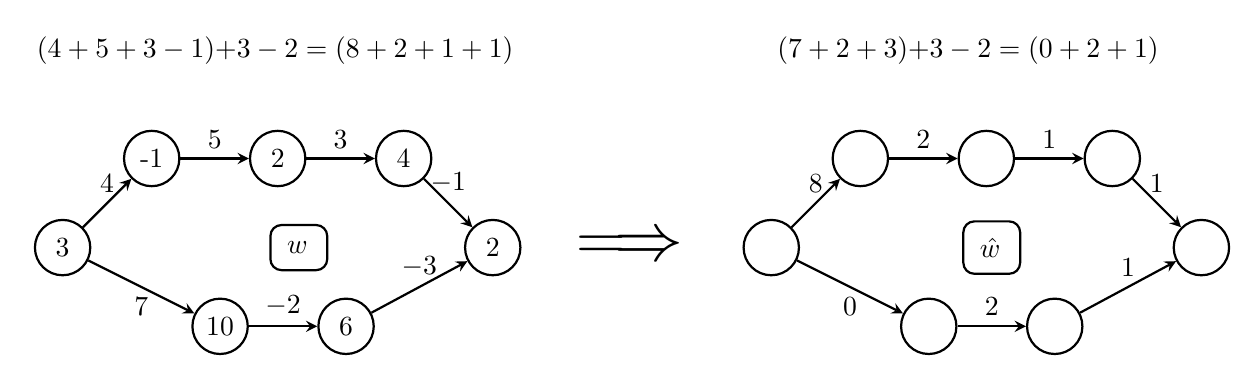
\begin{tikzpicture}[>=stealth, node distance=1.6cm, thick]
    
    \tikzstyle{v}=[circle, draw=black, fill=white, minimum size=20pt, inner sep=0pt]
    
    % ----------------------------
    % Left graph (original w)
    % ----------------------------
    \node[v] (a) at (0,0) {3};
    \node[v] (b) [above right of=a] {-1};
    \node[v] (c) [right of=b] {2};
    \node[v] (d) [right of=c] {4};
    \node[v] (e) [below right of=d] {2};
    
    \node[v] (f) at (2,-1) {10};
    \node[v] (g) [right of=f] {6};
    
    \draw[->] (a) -- (b) node[midway, above] {4};
    \draw[->] (b) -- (c) node[midway, above] {5};
    \draw[->] (c) -- (d) node[midway, above] {3};
    \draw[->] (d) -- (e) node[midway, above] {$-1$};
    
    \draw[->] (a) -- (f) node[midway, below] {7};
    \draw[->] (f) -- (g) node[midway, above] {$-2$};
    \draw[->] (g) -- (e) node[midway, above] {$-3$};
    
    \node[rectangle,rounded corners,draw=black,fill=white,
                inner sep=6pt,text width=0.3cm] 
                at (3,0)
                {$w$};
    
    \node at (2.7,2.5) {$(4 + 5 + 3 - 1) \red{+3-2} = (8 + 2 + 1 + 1)$};
    
    \node at (7.2,0) {\Huge $\Longrightarrow$};
    
    % ----------------------------
    % Right graph (\hat{w})
    % ----------------------------
    \node[v] (a2) at (9,0) {};
    \node[v] (b2) [above right of=a2] {};
    \node[v] (c2) [right of=b2] {};
    \node[v] (d2) [right of=c2] {};
    \node[v] (e2) [below right of=d2] {};
    
    \node[v] (f2) at (11,-1) {};
    \node[v] (g2) [right of=f2] {};
    
    \draw[->] (a2) -- (b2) node[midway, above] {8};
    \draw[->] (b2) -- (c2) node[midway, above] {2};
    \draw[->] (c2) -- (d2) node[midway, above] {1};
    \draw[->] (d2) -- (e2) node[midway, above] {1};
    
    \draw[->] (a2) -- (f2) node[midway, below] {0};
    \draw[->] (f2) -- (g2) node[midway, above] {2};
    \draw[->] (g2) -- (e2) node[midway, above] {1};
    
    \node[rectangle,rounded corners,draw=black,fill=white,
                inner sep=6pt,text width=0.3cm] 
                at (11.8,0)
                {$\hat{w}$};
    
    \node at (11.5,2.5) {$(7 + 2 + 3) \red{+ 3 - 2} = (0 + 2 + 1)$};
    
    \end{tikzpicture}
    \caption{Reweighting Example}
\end{figure}

\vspace{1em}

挑戰是在哪裡找 $h(i)$ 使得 $\hat{w}$ nonnegative?如果有了,我們就可以用 Dijkstra's algorithm 來解 All-Pairs Shortest Path Problem。

\newpage

\begin{idea}[Johnson's Technique: Finding $h(i)$]
    Following these steps:
    \begin{itemize}
        \item Let graph $H$ be obtained by adding a new vertex $s$ to $G$ and adding an edge $s_i$ of weight $0$ for each vertex $i$ of $G$.
        \begin{note}
            $H$ has no negative cycle iff $G$ has no negative cycle.
        \end{note}
        \item Let $h(i)$ be the distance from $s$ to $i$ in $H$, i.e. \[
            h(i) = d_H(s, i)
        \]
        \item The $d_H(s, i)$ can be computed using Bellman-Ford algorithm in $O(m + n)$ time.
    \end{itemize}
\end{idea}
\begin{proof}
    To see that $\hat{w}$ is nonnegative, observe the Figure 4.4.
    \begin{figure}[H]
        \centering
        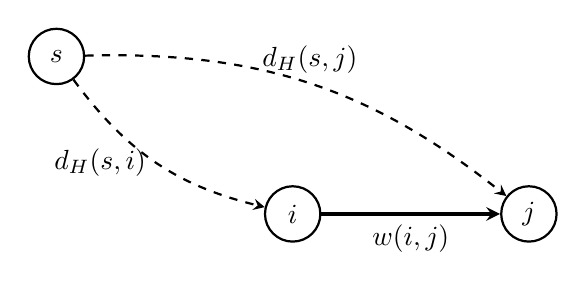
\begin{tikzpicture}[>=stealth, thick]
        \tikzstyle{v}=[circle, draw=black, fill=white, minimum size=20pt, inner sep=0pt]
        
        % Nodes
        \node[v] (o) at (0,2) {$s$};
        \node[v] (i) at (3,0) {$i$};
        \node[v] (j) at (6,0) {$j$};
        
        % Solid arrow i -> j
        \draw[->, very thick] (i) -- (j) node[midway, below] {$w(i,j)$};
        
        % Dotted curved arrow 0 -> i (lower)
        \draw[->, dashed, thick]
            (o) to[bend right=20] node[midway, left] {$d_H(s,i)$} (i);
        
        % Dotted curved arrow 0 -> j (upper)
        \draw[->, dashed, thick]
            (o) to[bend left=20] node[midway, above] {$d_H(s,j)$} (j);
        \end{tikzpicture}
        \caption{Proof of correctness of Johnson's Reweighting Technique}
    \end{figure}
    By observation, we have
    \begin{align*}
        \hat{w}(ij) &= w(ij) + h(i) - h(j) \\
        &\geq \underset{\red{\text{shortest $sj$-path which contain $i$}}}{(w(ij) + d_H(s, i))} - \underset{\blue{\text{shortest $sj$-path}}}{d_H(s, j)} \tag{Triangle Inequality} \\
        &= 0
    \end{align*}
\end{proof}


\begin{recall}
    Using Naive Solution with
    \begin{itemize}
        \item General edge weights: Bellman-Ford algorithm in $O(mn^2)$ time, which can be $\Theta(n^4)$ when $m = \Theta(n^2)$.
        \item Acyclic edge weights: Lawler's algorithm in $O(mn + n^2)$ time.
        \item Nonnegative edge weights: Dijkstra's algorithm in $O(mn + n^2\log n)$ time.
    \end{itemize}
    Using Floyd–Marshall’s DP algorithm in for general edge weights in $O(n^3)$ time.
\end{recall}

\newpage

\begin{idea}[Johnson's algorithm]
    Using Johnson's Reweighting Technique + Dijkstra's algorithm
    \begin{itemize}
        \item Obtain $h(i)$ for all vertex $i$ using Bellman-Ford algorithm in $O(mn)$ time, and get $\hat{w}$ from $w$ in $O(m)$ time.
        \item For each vertex $i$ of $G$, run Dijkstra's algorithm + Quake heap in \[
            O(m + n\log n)
        \]
        time on $G$ with edge weights $\hat{w}$ to compute $d_{\hat{G}}(i, j)$ for all $j \in V(G)$. Then obtain a shortest-paths tree of $G(\hat{G})$ rooted at $i$. 
        \item Compute $d_G(i, j)$ for all $j \in V(G)$ using \[
            d_G(i, j) = d_{\hat{G}}(i, j) + h(j) - h(i)
        \]
        in $O(n^2)$ time.
    \end{itemize}
    \begin{note}
        The running time is $O(mn + n^2\log n)$.
    \end{note}
\end{idea}


\chapter{Graph Theory: Maximum Flow Problem}

\begin{problem}[Maximum Flow Problem]
    Give 
    \begin{itemize}
        \item Input: A directed graph $G$ with edge capacities \[
            c: E(G) \to \mathbb{R}^+
        \], and two distinct vertices $s, t \in V(G)$ called \textbf{source} and \textbf{sink} respectively.
        \item Output: A ``$st$-flow'' with maximum ``(flow) value''.
    \end{itemize}
\end{problem}

\begin{com}
    在這個問題下我們允許 multiple/parallel edges 不需要合併成 simple network
\end{com}

\begin{definition*}
    Here are some definitions related to flows:
    \begin{definition}[$st$-flow]
        A $st$-flow is a function \[
            f: E(G) \to \mathbb{R}^+ \cup \{0\}
        \]
        that satisfies the following two conditions:
        \begin{itemize}
            \item Capacity constraint: \[
                f(e) \leq c(e) \quad \forall e \in E(G)
            \]
            \item Conservation law:
            \[
                \sum_{uv \in E(G)} f(uv) = \sum_{vu \in E(G)} f(vu) \quad \forall v \in V(G) \setminus \{s, t\}
            \]
        \end{itemize}
    \end{definition}
    \begin{definition}[Flow value]
        The flow value of a flow $f$ is defined as
        \[
            |f| = \sum_{sv \in E(G)} f(sv) - \sum_{us \in E(G)} f(us)
        \]
    \end{definition}
\end{definition*}

\newpage

\section{Ford–Fulkerson's Algorithm}

\begin{intuition}
    We can reduce the Maximum Flow Problem into reachability problem for a sequence of \textbf{residual graphs} $R$. 
\end{intuition}    

\begin{definition}[Residual Graph]
    The residual graph $R(f)$ with respect to a flow $f$ of $G$ with $V(G) = V(R(f))$ is defined as follows for each $uv \in E(G)$:
    \begin{itemize}
        \item If $f(uv) < c(uv)$, then $R(f)$ contains an edge \red{$uv$} with capacity \[
            c_{R(f)}(uv) = c(uv) - f(uv)
        \]
        \item If $f(uv) > 0$, then $R(f)$ contains a reverse edge \blue{$vu$} with capacity \[
            c_{R(f)}(vu) = f(uv)
        \]
    \end{itemize}
\end{definition}

\begin{com}[1]
    $R(f)$ 跟 $G$ 一樣,所有 $c(uv)$ 都會是正的,不會是 0 或負的。
\end{com}

\begin{com}[2]
    $G$ 最多讓 $flow$ 增加 2 倍,因為每條邊 $uv$ 在 $R(f)$ 裡面最多會有兩條邊:\red{$uv$} 和 \blue{$vu$},只要兩個條件都達成。
\end{com}

\begin{lemma}
    For any $st$-flow $f$ in $G$, we have the following properties:
    \begin{itemize}
        \item If $d_{R(f)} = \infty$, then $f$ is a maximum $st$-flow in $G$.
        \item If $d_{R(f)} < \infty$, and $g$ is an $st$-flow in $R(f)$, then $f + g$ remains an $st$-flow in $G$, where \[
            (f + g)(uv) = f(uv) + g(uv) - g(vu), \quad \forall uv \in E(G)
        \]
    \end{itemize}
    \begin{note}
        這裡的 $g(uv), g(vu)$ 都是由原始的 $uv$-edge 產生的,因此原始圖若有 $vu$ edge 必須分開處理,不能混在上面兩個式子裡面。
    \end{note}
\end{lemma}
\begin{proof}
    % Proof of first property
    Let $f'$ be the maximum $st$-flow in $G$, but not $f$. We defined $h$ as follows:
    \[
        h(uv) = f(uv) - f'(uv), \quad \forall uv \in E(G)
    \]
    Since $f$ and $f'$ are both $st$-flows in $G$, we have conservation law for $f$ and $f'$, so $h$ satisfies conservation law as well.
    \[
        \sum_{uv \in E(G)} h(uv) = \sum_{vu \in E(G)} h(vu) \quad \forall v \in V(G) \setminus \{s, t\}
    \]
    Now consider some vertex $x, y, z \in V(G) \setminus \{s, t\}$. If $h(xy) > 0$, because $h$ satisfies conservation law, there must exist some $h(yz) > 0$. Continuing this process, we can find a path $P$,
    \[
        P = s \to v_1 \cdots \to v_k \to t \quad \text{such that } h(v_i v_{i+1}) > 0 \quad \forall i = 0, 1, \cdots, k
    \] 
    If $h(uv) > 0$, we have \[
        f(uv) > f'(uv) \geq 0 \tag{1}
    \] we know $f'(uv)$ can not exceed $c(uv)$, so\[ f'(uv) \leq c(uv) \tag{2} \] by (1) and (2), we have \[ f(uv) < c(uv) \] which means \[ c_{R(f)}(uv) = c(uv) - f(uv) > 0 \]
    Therefore, all edges in $R(f)$ along path $P$ have positive capacities. Which is a $st$-path in $R(f)$, contradicting the assumption that $d_{R(f)} = \infty$.

    Now we start to prove the second property. We need to show that $f + g$ satisfies capacity constraint and conservation law.
    \begin{itemize}
        \item Capacity constraint: For any $uv \in E(G)$, we havee some constraint:
        \begin{itemize}
            \item $g(uv) < c_{R(f)}(uv) = c(uv) - f(uv) \leq c(uv)$
            \item $g(vu) \leq c_{R(f)}(vu) = f(uv)$
        \end{itemize}
        to maximize $(f + g)(uv)$, we set $g(uv)$ to its maximum and $g(vu)$ to its minimum, so we have
        \[
            (f + g)(uv) = f(uv) + g(uv) - g(vu) \leq f(uv) + (c(uv) - f(uv)) - 0 = c(uv)
        \]
        \item Conservation law: For any $v \in V(G) \setminus \{s, t\}$, we have
        \begin{align*}
            \sum_{uv \in E(G)} (f + g)(uv) 
            &= \ \sum_{uv \in E(G)} (f(uv) + g(uv) - g(vu)) \\ 
            &= \sum_{uv \in E(G)} f(uv) + \sum_{uv \in E(G)} g(uv) - \sum_{uv \in E(G)} g(vu) \\ 
            &= \sum_{uv \in E(G)} f(uv) + 0 \tag{by conservation law of $g$} \\ 
            &= \sum_{vu \in E(G)} f(vu) \tag{by conservation law of $f$} \\
            &= \sum_{vu \in E(G)} (f(vu) + g(vu) - g(uv)) \tag{by conservation law of $g$} \\
            &= \sum_{vu \in E(G)} (f + g)(vu)
        \end{align*}
    \end{itemize}
\end{proof}

\newpage

\begin{algorithm}[H]
    \DontPrintSemicolon
    \SetAlgoLined
    \KwIn{A flow network $G=(V,E)$ with capacity $c(u,v)$; source $s$; sink $t$.}
    \KwOut{A maximum flow $f$.}

    Initialize $f(u,v) \gets 0$ for all $(u,v)\in E$\;
    Compute residual capacity 
    \[
        c_{R(f)}(uv) = \begin{cases}
            c(uv) - f(uv) & \text{if } f(uv) < c(uv)  \\
            f(uv) & \text{if } f(uv) > 0
        \end{cases}
    \]
    \;

    \While{$\exists\ st-\text{augmenting path } P$ in  $R(f)$}{
        Obtain an $st$-path $P$ of $R(f)$, let \(
            q = \min_{uv \in P} c_{R(f)}(u,v)
        \)\;
        Obtain a $st$-flow $g$ of $R(f)$ by setting \[
            g(uv) = \begin{cases}
                q & \text{if } uv \in P \\
                0 & \text{otherwise}
            \end{cases}
        \]\;
        Update flow $f \gets f + g$\;
    }
    \Return $f$\;
    \caption{Ford-Fulkerson Algorithm}
\end{algorithm}
\begin{proof}[correctness]
    We separately prove three things:
    \begin{itemize}
        \item Initialization: $f$ is a valid flow in $G$ with value $0$.
        \item According to Lemma 5.1.1(關鍵觀察): In every round $g$ is a valid flow in $R(f)$, so $f + g$ is a valid $st$-flow in $G$.
        \item Termination: When the algorithm terminates, $d_{R(f)}(s,t) = \infty$, so by \blue{Lemma 5.1.1}, $f$ is a maximum $st$-flow in $G$.
    \end{itemize}
    Proof complete.
\end{proof}

\begin{definition}[augmenting path]
    In Ford-Fulkerson algorithm, obtain a $st$-path $P$ of $R(f)$, let \(
        \displaystyle q = \min_{uv \in P} c_{R(f)}(u,v)
    \). The path $P$ is called an \textbf{augmenting path} with respect to flow $f$.
\end{definition}

\begin{definition}[saturating flow]
    In Ford-Fulkerson algorithm, obtain a $st$-flow $g$ of $R(f)$ by setting \[
        g(uv) = \begin{cases}
            q & \text{if } uv \in P \\
            0 & \text{otherwise}
        \end{cases}
    \]. The flow $g$ is called a \textbf{saturating flow} with corresponding to $P$.
\end{definition}

